
% Szkielet dla pracy inżynierskiej pisanej w języku polskim.

\documentclass[polish,masters,a4paper,twoside]{ppfcmthesis}


\usepackage[utf8]{inputenc}
\usepackage[OT4]{fontenc}
\usepackage{algorithm}
\usepackage{algorithmic}
\usepackage{listings}

\usepackage{rotating}
\usepackage{pdfpages}

% Authors of the thesis here. Separate them with \and
\author{Wiktor Latanowicz \album{66271}}
\authortitle{}                                        % Do not change.
\title{Framework do tworzenia aplikacji internetowych uruchamianych w środowisku przeglądarki}                   % Note how we protect the final title phrase from breaking
\ppsupervisor{dr inż. Rafał Różycki} % Your supervisor comes here.
\ppyear{2013}                                         % Year of final submission (not graduation!)

\lstset{basicstyle=\small, breakindent=40pt, breaklines}
\lstdefinelanguage[Objective]{C}[GNU99]{C}
  {morekeywords={@catch,@class,@encode,@end,@finally,@implementation,%
      @interface,@private,@protected,@protocol,@public,@selector,%
      @synchronized,@throw,@try,BOOL,Class,IMP,NO,Nil,SEL,YES,_cmd,%
      bycopy,byref,id,in,inout,nil,oneway,out,self,super,%
      % The next two lines are Objective-C 2 keywords.
      @dynamic,@package,@property,@synthesize,readwrite,readonly,%
      assign,retain,copy,nonatomic%
      },%
   moredirectives={import}%
  }%
\lstdefinelanguage[GNU99]{C}[99]{C}
  {morekeywords={asm,__asm__,__extension__,typeof,__typeof__}%
  }%
\lstdefinelanguage[99]{C}%
  {morekeywords={_Bool,_Complex,_Imaginary,auto,break,case,char,%
      const,continue,default,do,double,else,enum,extern,float,for,%
      goto,if,inline,int,long,register,restrict,return,short,signed,%
      sizeof,static,struct,switch,typedef,union,unsigned,void,volatile,%
      while},%
   sensitive,%
   morecomment=[s]{/*}{*/},%
   morecomment=[l]//,%
   morestring=[b]",%
   morestring=[b]',%
   moredelim=*[directive]\#,%
   moredirectives={define,elif,else,endif,error,if,ifdef,ifndef,line,%
      include,pragma,undef,warning}%
  }[keywords,comments,strings,directives]%
  
  
\begin{document}

% Front matter starts here
\frontmatter\pagestyle{empty}%
\maketitle\cleardoublepage%

% Blank info page for "karta dyplomowa"
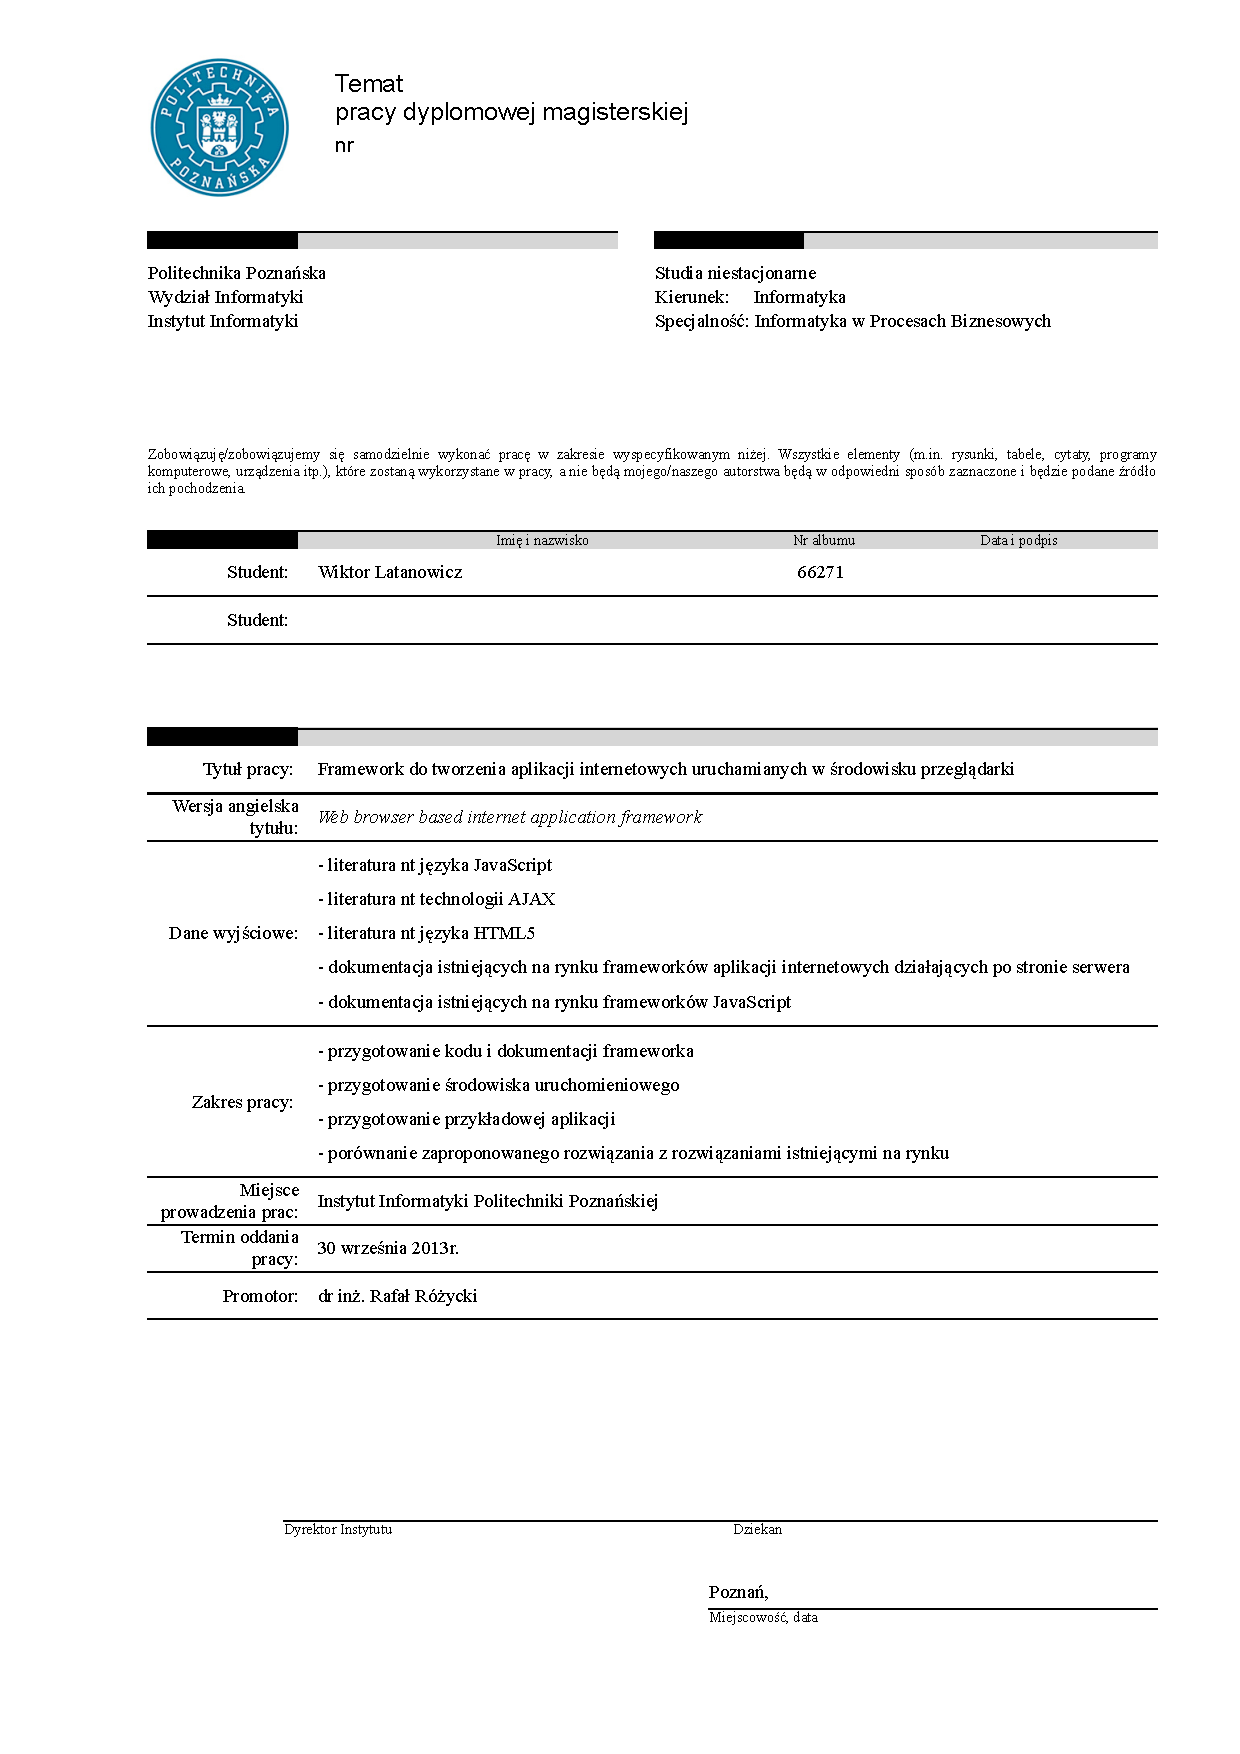
\includepdf{figures/karta}
\cleardoublepage%

% Table of contents.
\pagenumbering{Roman}\pagestyle{ppfcmthesis}%
\tableofcontents* \cleardoublepage%

% Main content of your thesis starts here.
\mainmatter%

\chapter{Wstęp}



\chapter{Podstawy teoretyczne}


\chapter{Projekt i implementacja systemu}

\chapter{Testowanie}


\chapter{Zakończenie}


\section{Podsumowanie}


\cleardoublepage\appendix%

\chapter{Diagram klas całego systemu}


\nocite{*}

% Bibliography (books, articles) starts here.
\bibliographystyle{plalpha}{\raggedright\sloppy\small\bibliography{bibliography}}

% Colophon is a place where you should let others know about copyrights etc.
\ppcolophon

\end{document}
